%%%%%%%%%%%%%%%%%%%%%%%%%%%%%%%%%%%%%%%%%
% Thin Sectioned Essay
% LaTeX Template
% Version 1.0 (3/8/13)
%
% This template has been downloaded from:
% http://www.LaTeXTemplates.com
%
% Original Author:
% Nicolas Diaz (nsdiaz@uc.cl) with extensive modifications by:
% Vel (vel@latextemplates.com)
%
% License:
% CC BY-NC-SA 3.0 (http://creativecommons.org/licenses/by-nc-sa/3.0/)
%
%%%%%%%%%%%%%%%%%%%%%%%%%%%%%%%%%%%%%%%%%

%----------------------------------------------------------------------------------------
%   PACKAGES AND OTHER DOCUMENT CONFIGURATIONS
%----------------------------------------------------------------------------------------

\documentclass[11pt]{article} % Font size (can be 10pt, 11pt or 12pt) and paper size (remove a4paper for US letter paper)

\usepackage[utf8]{inputenc} % Set utf8 code
\usepackage[protrusion=true,expansion=true]{microtype} % Better typography
\usepackage[portuguese]{babel}
\usepackage{graphicx} % Required for including pictures
\usepackage{wrapfig} % Allows in-line images
\usepackage[pagebackref]{hyperref}

\usepackage{mathpazo} % Use the Palatino font
\usepackage[T1]{fontenc} % Required for accented characters

\usepackage{wallpaper}
\usepackage[font={color=white,bf},figurename=Fig.,labelfont={it}]{caption}
\usepackage{lipsum, xcolor, etoolbox, footmisc, bigfoot}

\usepackage{tabu}
\hypersetup{
    colorlinks=false,
    pdfborder={0 0 0},
}


\linespread{1.05} % Change line spacing here, Palatino benefits from a slight increase by default

\makeatletter
\renewcommand\@biblabel[1]{\textbf{#1.}} % Change the square brackets for each bibliography item from '[1]' to '1.'
\renewcommand{\@listI}{\itemsep=0pt} % Reduce the space between items in the itemize and enumerate environments and the bibliography

\renewcommand{\maketitle}{ % Customize the title - do not edit title and author name here, see the TITLE block below


\begin{center} % Right align
{\LARGE\@title} % Increase the font size of the title

\vspace{20pt} % Some vertical space between the title and author name

\end{center}
}

\patchcmd{\ps@plain}{\thepage}{\textcolor{white}{\thepage}}{}{}
\makeatother

\begin{document}

\ThisTileWallPaper{\paperwidth}{\paperheight}{res/wallpaper_header.jpg}
\color{white}
\pagestyle{plain}
\def\footnotelayout{\color{white}}
\renewcommand\thefootnote{\textcolor{white}{\arabic{footnote}}}
\begin{titlepage}
 \vfill
  \begin{center}
   {\large \textbf{Tiamat}} \\
   {\large \textbf{Babel}}\\
   {\large \href{mailto:tiamatbabel@gmail.com}{tiamatbabel@gmail.com}}\\[6cm]


   {\Large \textbf{GDD}}\\
   {\Large Versão 0.6}\\[6cm]

   \hspace{.45\textwidth} %posiciona a minipage
  \vfill

\vspace{2cm}

\large \textbf{Brasília}

\large \textbf{Abril de 2015}
\end{center}
\end{titlepage}
\newpage

\tableofcontents

\newpage

%----------------------------------------------------------------------------------------
%   DOC BODY
%----------------------------------------------------------------------------------------

\TileWallPaper{\paperwidth}{\paperheight}{res/wallpaper_body.jpg}
\color{white}

\section*{Tabela de Revisão}


\begin{table}[h]

  \taburulecolor{white}
  \color{white}
\begin{tabu}{|l|l|p{60mm}|l|}

\hline 
\textbf{Versão}     & \textbf{Data}     & \textbf{Descrição}                                    & \textbf{Autor}    \\ \hline
0.1                 & 14/04/2015        & Versão inicial                                        & Álex Mesquita     \\ \hline
0.2                 & 15/04/2015        & Requisitos Tecnológicos                               & Álex Mesquita     \\ \hline
0.3                 & 15/04/2015        & Revisão ortográfica                                   &                   \\ \hline
0.4                 & 25/04/2015        & Front End                                             & Álex Mesquita     \\ \hline
0.5                 & 29/04/2015        & Atualização da imagem de fundo                        & Álex Mesquita     \\ \hline
0.5.1               & 21/05/2015        & Criação das mecânicas do jogo - Exploração vertical   & Jefferson Xavier  \\ \hline
0.5.2               & 21/05/2015        & Criação da Mecânica Exploração horizontal             & Jefferson Xavier  \\ \hline
0.6                 & 21/05/2015        & Finalização das Mecânicas                             & Jefferson Xavier  \\ \hline
\end{tabu}
\end{table}

\newpage

\section{Objetivo do jogo}

\paragraph{}Jogo singleplayer com temática \textit{Sci-fi}, onde a raça humana vagueia pelo universo à procura de um novo planeta habitável, pois a humanidade extinguiu alguns recursos essenciais que a Terra continha. Após receber um sinal, a raça humana desloca sua nave espacial para um planeta desconhecido à procura desse sinal e acaba encontrando uma torre que definitivamente não podia ter sido construída por humanos. O desafio do jogador será explorar essa torre afim de descobrir seus mistérios, no entanto o jogador deverá explorar o planeta para encontrar recursos que poderão evoluir as habilidades dos personagens ou serem utilizados para construir equipamentos para facilitar a exploração da torre.


\section{Visão geral}

\paragraph{}O jogo se inicia na base de exploração construída próxima à torre a ser explorada. Nesta base haverá algumas construções essenciais para que o jogador possa evoluir os seus personagens, possibilitando assim montar uma estratégia de exploração da torre e dos recursos contidos no planeta.

\paragraph{}A partir da visão de sua base o jogador poderá transitar pelos cenários da torre e da superfície do planeta. Para acessar a torre o jogador deverá clicar sobre um botão de missões na torre que estará disponível no cenário da base. Para retornar à sua base, o jogador deverá concluir ou abortar a missão. Do mesmo modo, para acessar a superfície do planeta, o jogador deverá clicar sobre um botão de missões sobre a superfície da torre que também estará disponível no cenário da base. Ao abrir o cenário da superfície, o jogador poderá selecionar qual missão este irá executar, neste cenário terá um botão para se retornar à base.

\paragraph{}O objetivo do jogo é descobrir o propósito da torre e quem construiu esse edifício misterioso. Ao entrar em contato com tal ser, o que ocorreria em seguida? Uma Guerra? Trocas de experiências? Para isso o jogador deverá explorar todos os níveis da torre com os seus personagens. E para facilitar a exploração, será possível coletar \textit{Data points}\footnote{Pontos que serão obtidos através da execução de missões}, podendo assim evoluir os personagens, facilitando o seu desempenho durante as missões na torre. 

\subsection{Mecânicas do Jogo}
\paragraph{}Esta sessão apresentará todas as mecânicas existentes no jogo, com detalhes sobre as explorações horizontal e vertical, Base, Combates, Eventos e Relógio.

\subsubsection{Exploração Vertical}
\paragraph{}A Exploração Vertical consiste na exploração da Torre. Que se vai dar em um formato clássico de Dungeon Crawl, a vista em primeira pessoa e a imersão dada contribui para a experiência de exploração e incerteza, já que a Torre terá corredores labirintíticos.

\paragraph{}Quando o jogador mostra interesse em explorar a Torre, ele deve antes escolher uma equipe que consiste em 4 Heróis e 1 Drone. Depois de selecionado a equipe e o andar que se deseja explorar, as mecânicas da Exploração Vertical começam a agir.

\begin{enumerate}
  \item \textbf{Movimentação}: A Movimentação dentro da Torre é medida por meio de quadrados que compõem o mapa do andar da Torre. Porém, entre um quadrado e outro existem algumas coisas que podem impedir a movimentação da equipe para aquela dada direção;
  \item \textbf{Eventos}: Os Eventos são conflitos que aparecem ao jogador, e que devem ser resolvidos para que o jogador consiga progredir no jogo. Eles são conflitos que aparecem, propondo um desafio, e são dadas opções ao jogador para que ele possa resolver o dado desafio. Os Eventos podem ser de tipos diferentes, que são: Combates, que é quando inimigos aparecem para o jogador em algum ponto específico da exploração da torre, nesse caso esses inimigos devem ser derrotados pela equipe. Objetos, podem aparecer durante a exploração para que o jogador. Portas, são pontos de divisão do andar da torre, podem servir para separar corredores e salas, por exemplo, podem ser secretas ou inacessíveis também até certo momento da exploração, até que algum inimigo seja derrotado, por exemplo.
\end{enumerate}
\newpage

\begin{figure}[!htp]
\centering
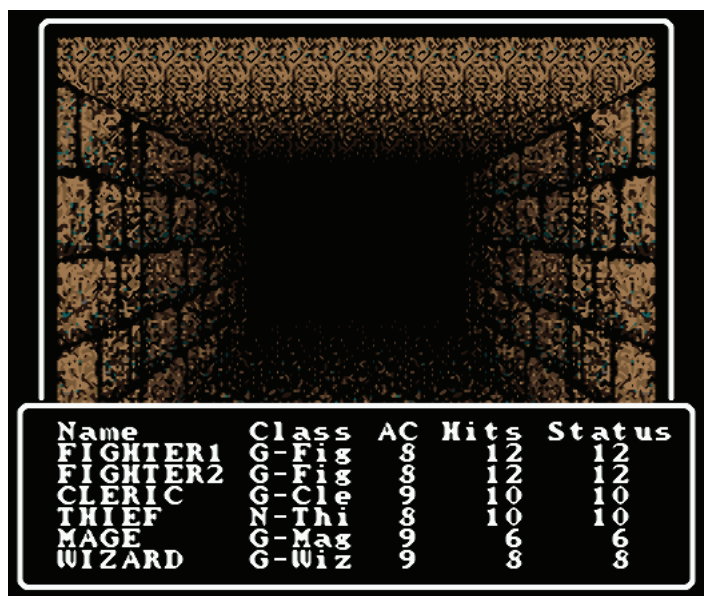
\includegraphics[scale=0.3]{res/Dungeon_Crawler.png}
\caption{Exploração Vertical - Exemplo de Dungeon Crawl}
\label{Exploração Vertical - Exemplo de Dungeon Crawl}
\end{figure}

\subsubsection{Exploração Horizontal}
\paragraph{}A Exploração Horizontal vem como suporte para a mecânica de Exploração Vertical, que é por onde a maioria da experiência do jogo será passada. É a exploração do planeta, que tem como principal função ser uma fonte de recursos brutos que serão necessários para a construção e manutenção da sua base de operações, enfatizando o senso de necessidade e sobrevivência da espécie.

\begin{enumerate}
  \item \textbf{Espaço}: A Exploração Horizontal se dá na superfície do planeta colonizado, na região que circunda a misteriosa Torre. Os recursos serão extraídos dos locais próximos.
  \item \textbf{Locais}: Estes locais estarão posicionados em uma malha virtual abstrata, posicionadas nos vértices desta mesma malha. A cada local explorado, é revelado no mapa do planeta todos os locais que ligam aquele local na malha, aumentando as possibilidades e locais de exploração.
  \item \textbf{Resolução e recompensas}: Todo local de exploração terá algum desafio para ser resolvido e em caso de sucesso o jogador ganhará recursos que poderão ser usados para evolução de sua base. Os desafios podem variar e cabe ao jogador formar a melhor estratégia e mandar a melhor equipe de acordo com as necessidades para cumprir esses objetivos.
\end{enumerate}

\begin{figure}[!htp]
\centering
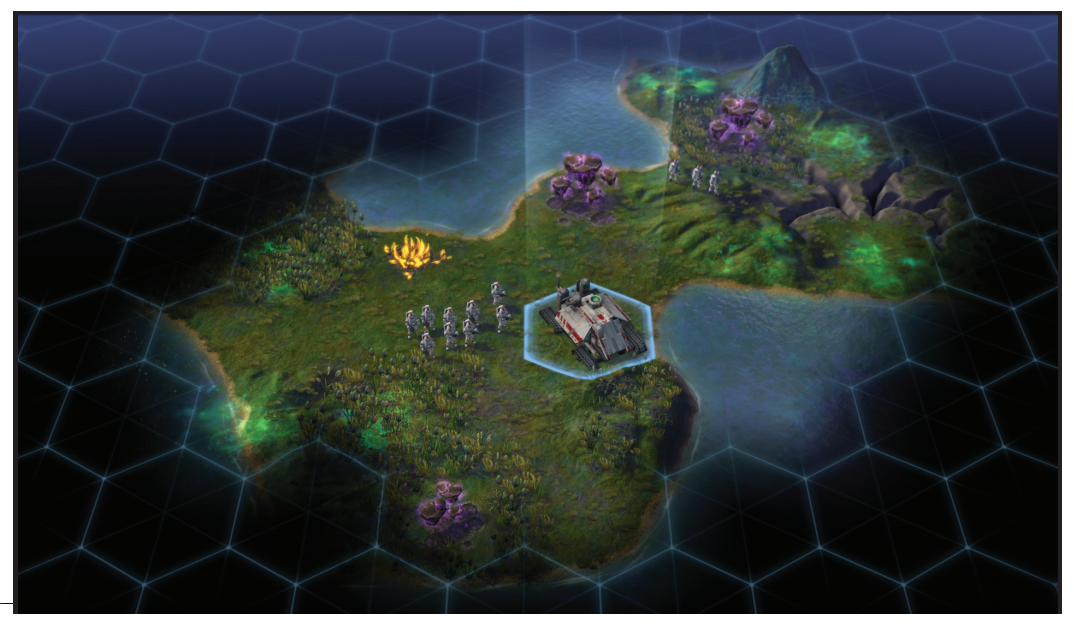
\includegraphics[scale=0.3]{res/resources.png}
\caption{Exemplo de Exploração Horizontal}
\label{Exemplo de Exploração Horizontal}
\end{figure}

\subsection{Base Building}
\paragraph{}Além da exploração da torre e do planeta o jogo também deve conter uma base principal, essa é a base onde o jogador evolui seus personagens, atributos, construções e tecnologias, tudo é evoluído a partir do que é ganho nas explorações vertical e horizontal. Ao todo são sete tipos de construções que existirão na base.

\begin{enumerate}
  \item \textbf{Fundição/Fábrica}: Criação de equipamentos e drones;
  \item \textbf{Clínica Genética}: Cura de personagens feridos em uma dada exploração e dá upgrade nos atributos passivos dos personagens, como defesa, vida e quantidade de dano;
  \item \textbf{Quartel General}: Atualização das unidades militares;
  \item \textbf{Laboratório}: Atualização das unidades tecnológicas;
  \item \textbf{Centro de Inteligência}: Atualização das unidades psiônicas;
  \item \textbf{Centro de Pesquisa}: Pesquisa de novos itens;
  \item \textbf{Centro de Comando}: Selecionar missões e contratar novos personagens.
\end{enumerate}
\newpage

\begin{figure}[!htp]
\centering
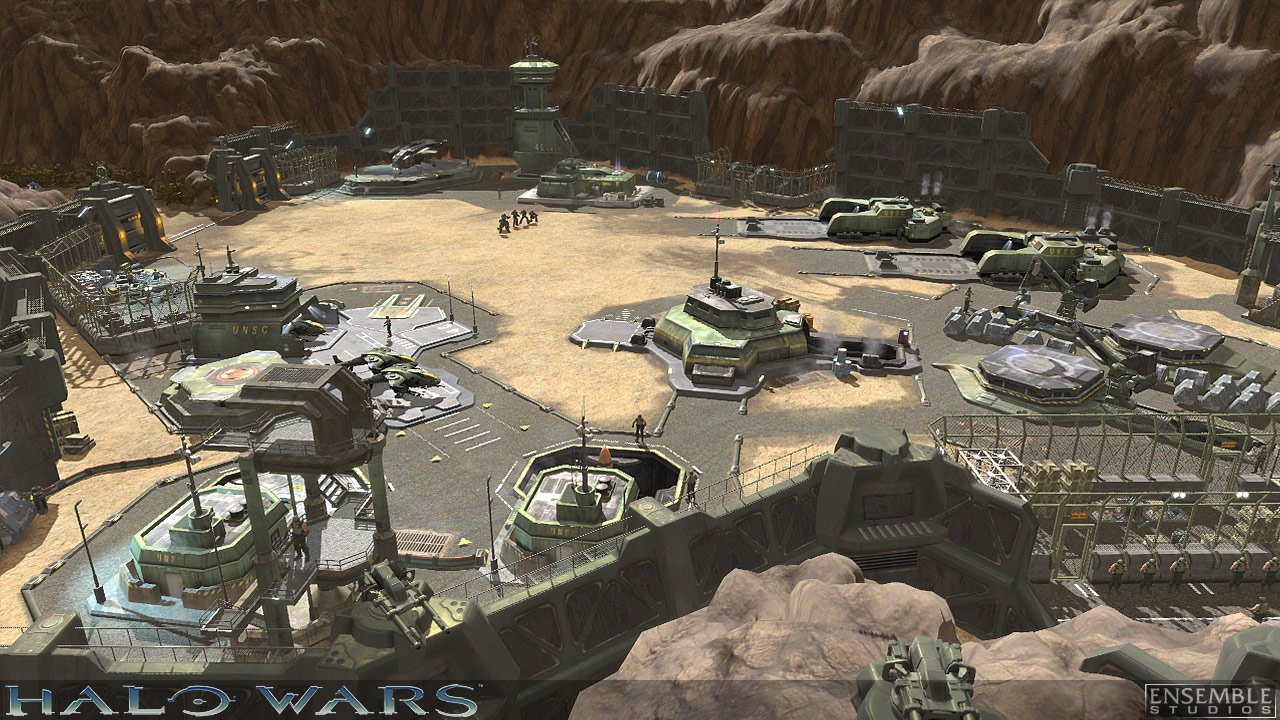
\includegraphics[scale=0.3]{res/base_building.png}
\caption{Exemplo de Base Building}
\label{Exemplo de Base Building}
\end{figure}

\section{Esquema de controle e interface com o usuário}

\paragraph{}Na exploração vertical, no interior da torre, esta será em primeira pessoa, sendo que serão utilizadas as teclas destacadas na figura a seguir:\\

\begin{figure}[!htp]
\centering
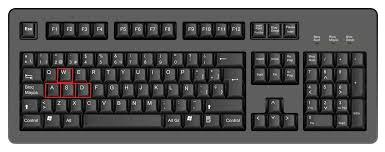
\includegraphics[scale=0.75]{res/keyboard.jpg}
\caption{Teclas utilizadas}
\label{Teclado}
\end{figure}

\paragraph{}Onde a tecla ''w'' irá movimentar o jogador para frente, a tecla ''s'' irá movimentar o jogador para trás, a tecla ''a'' irá rotacionar o jogador $90\,^{\circ}$ para a esquerda e a tecla ''d'' irá rotacionar o jogador $90\,^{\circ}$ para a direita. A tecla ''e'' será utilizada para interação dos objetos com o personagem.

\paragraph{}Na exploração horizontal, a superfície do planeta, o jogador irá usar o \textit{mouse} para navegar na superfície, utilizando o botão esquerdo para selecionar objetos e executar todas as ações na base e superfície do planeta. Na exploração vertical, no interior da torre, o botão esquerdo servirá para realizar a ação principal do personagem.

\begin{figure}[!htp]
\centering
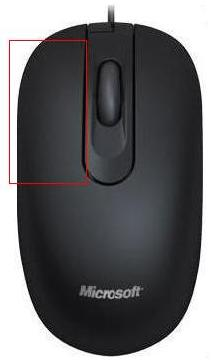
\includegraphics[scale=0.4]{res/mouse.jpg}
\caption{Mouse}
\label{Mouse}
\end{figure}

\section{Front End}

\paragraph{} O \textit{Front End} representa as tela que serão carregadas assim que o jogo é iniciado. A seguir serão ilustradas cada uma das telas que serão apresentadas ao iniciar o \textbf{Babel}.

\paragraph{} A logo a seguir representa a empresa responsável por desenvolver o jogo.

\begin{figure}[!htp]
\centering

\includegraphics[scale=0.6]{res/tiamat_logo.png}
\caption{Logo da Tiamat}
\label{Logo da Tiamat}
\end{figure}

\paragraph{} A logo a seguinte representa a API utilizada durante o desenvolvimento.

\begin{figure}[!htp]
\centering

\includegraphics[scale=0.6]{res/Sdl-logo.png}
\caption{Logo da SDL}
\label{Logo da SDL}
\end{figure}

\paragraph{} A imagem a seguir representa a classificação indicativa para o jogadores.

\newpage

\begin{figure}[!htp]
\centering

\includegraphics[scale=0.5]{res/classification.png}
\caption{Classificação Indicativa}
\label{Classificação Indicativa}
\end{figure}

\section{Requisitos Tecnológicos}

\begin{figure}[tb]
\begin{center}
  
\includegraphics[scale=0.3]{res/cubase-Logo.png} \quad
  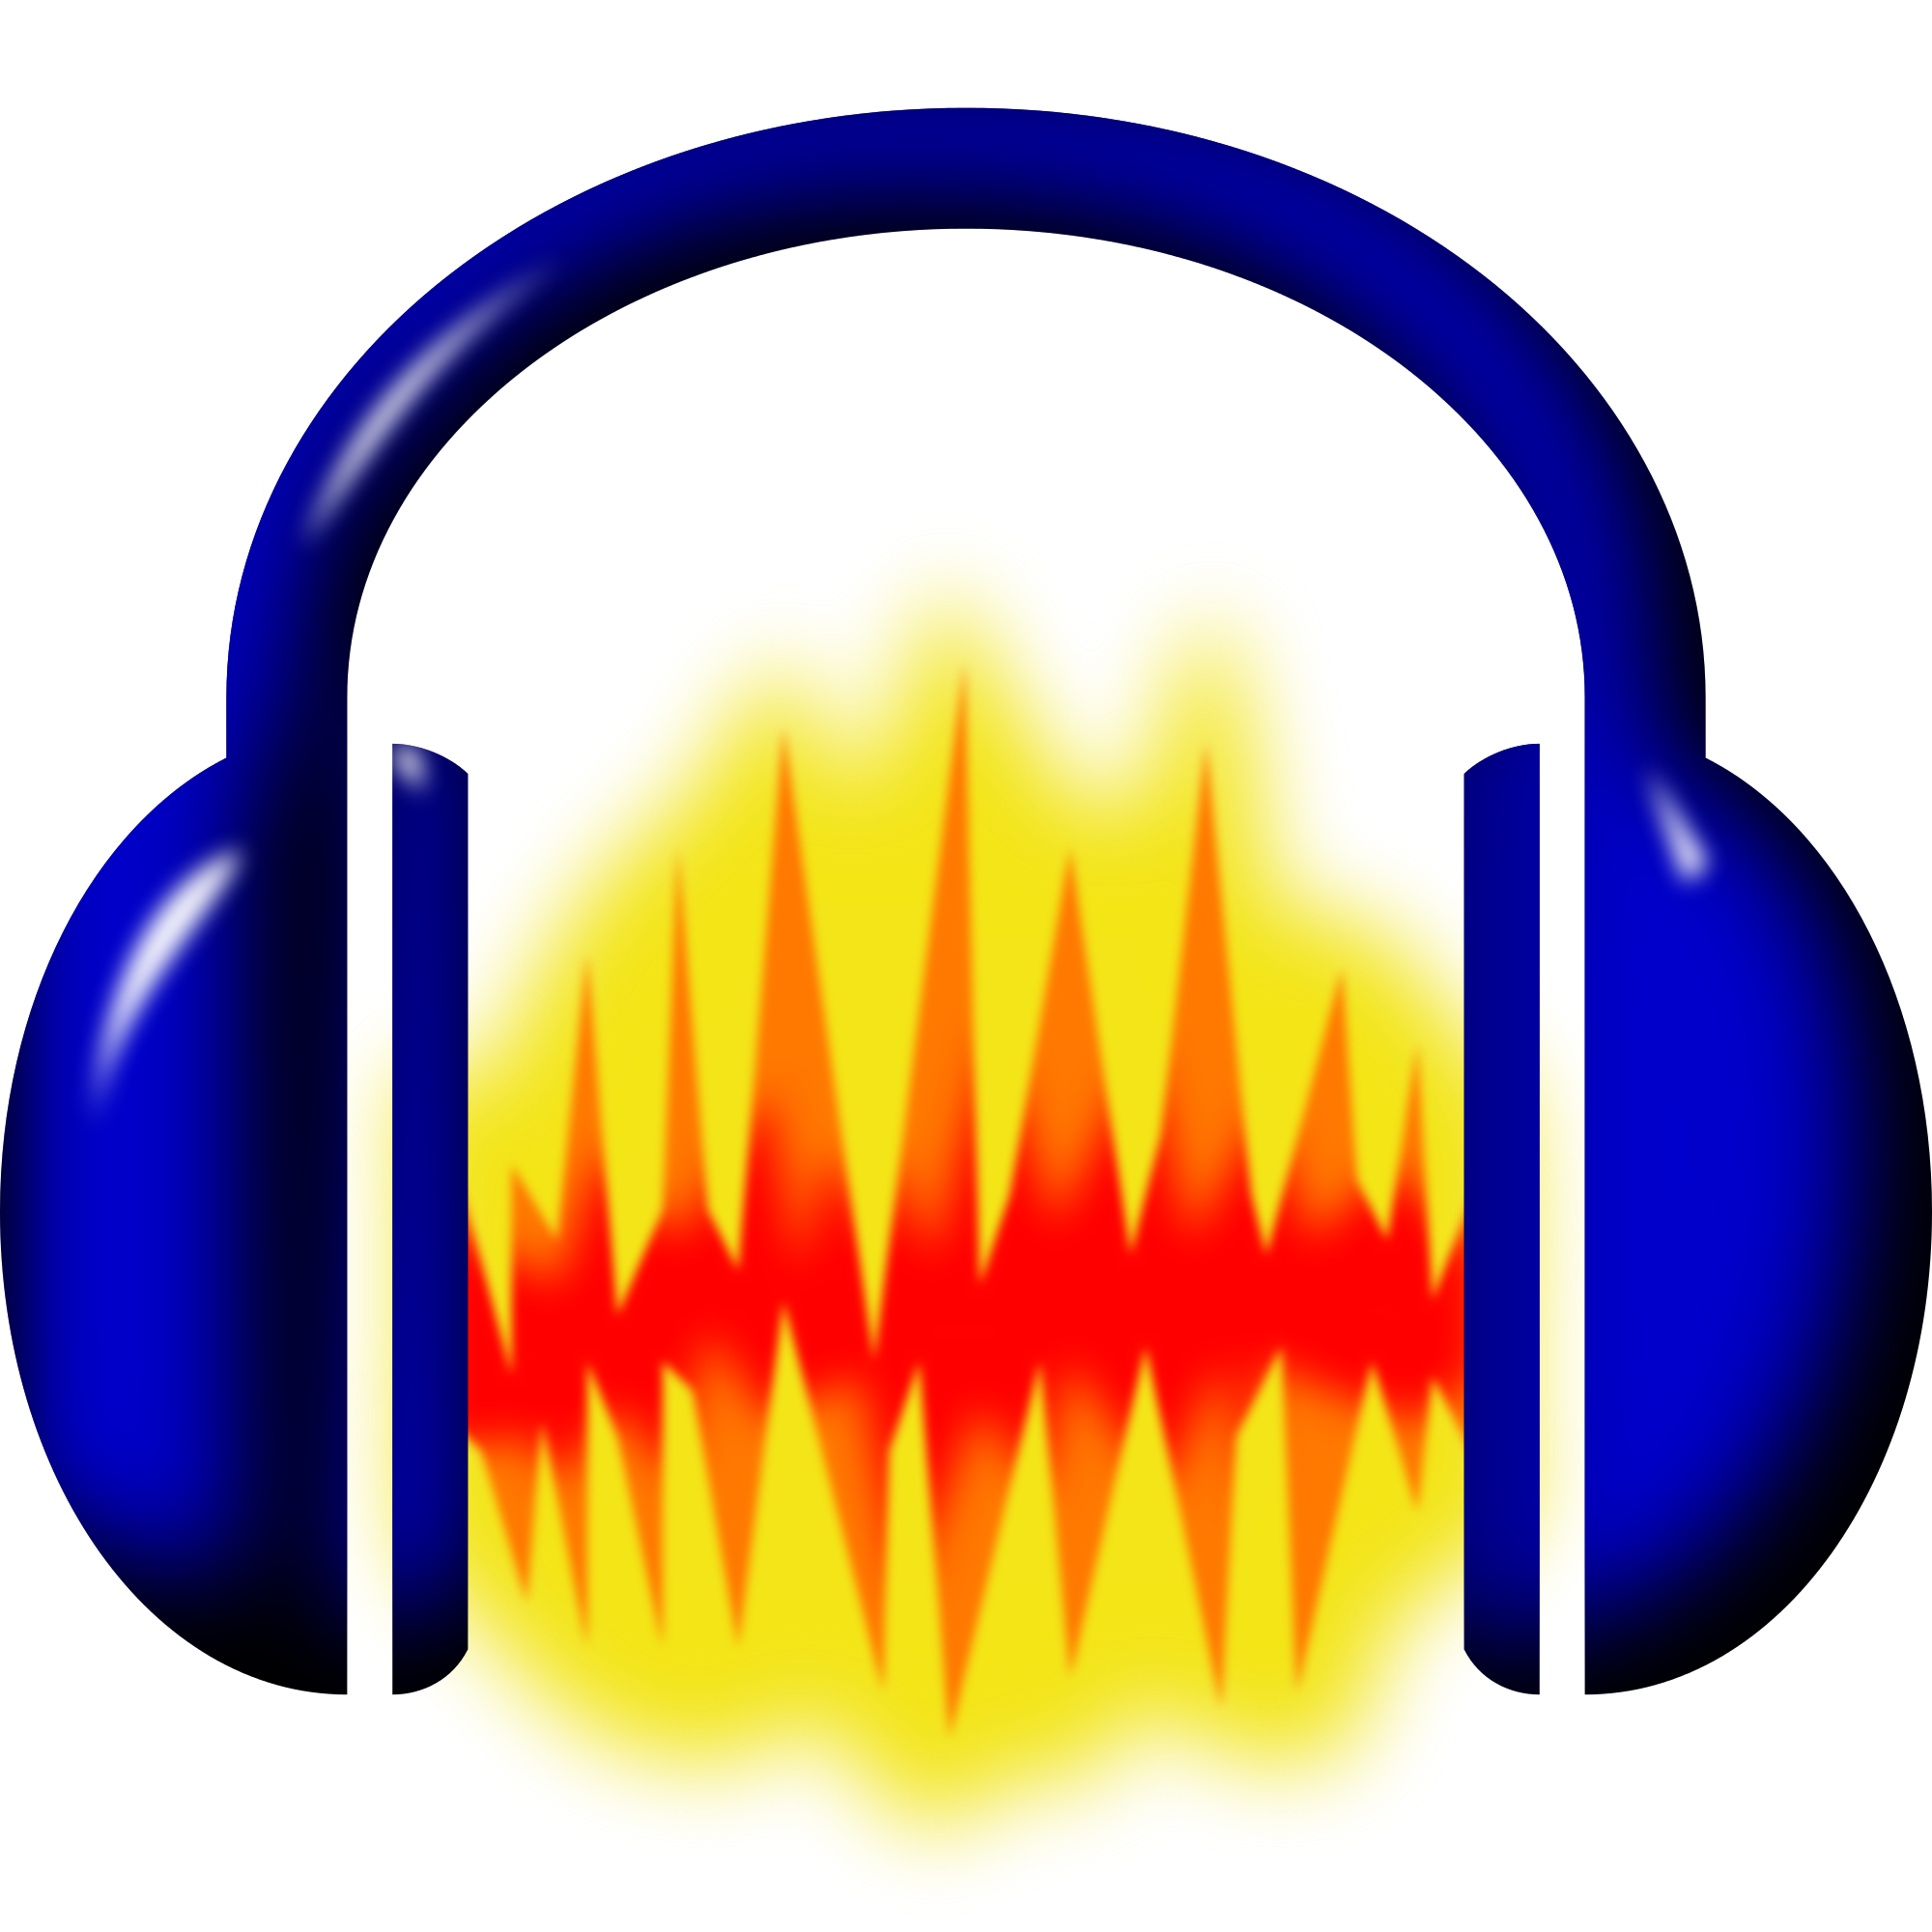
\includegraphics[scale=0.04]{res/audacity.png} \quad
  
\includegraphics[scale=0.3]{res/adobe_illustrator.png} \quad
  
\includegraphics[scale=0.25]{res/Sdl-logo.png} \quad
  
\includegraphics[scale=0.3]{res/Sublime_Text_Logo.png} \quad
  
\includegraphics[scale=0.2]{res/cpp.png} \quad
  
\includegraphics[scale=0.13]{res/git.png} \quad
  
\includegraphics[scale=0.15]{res/lua.png} \quad
  
\includegraphics[scale=0.4]{res/GDB.png} \quad
  
\includegraphics[scale=0.16]{res/linux.png} \quad
  
\includegraphics[scale=0.35]{res/GCC.png} \quad
  
\includegraphics[scale=0.05]{res/windows.png} \quad
\caption{Requisitos Tecnológicos} \label{gdimotes}
\end{center}
\end{figure}

\end{document}
